\documentclass[border=12pt, multi, tikz]{standalone}
%\usepackage{blocks}
% \usepackage[top=4cm,left=2cm]{geometry}
\usepackage[fontsize=14pt]{fontsize}
\usepackage{import}
\subimport{../../layers/}{init}
%\usepackage{optics}
\usetikzlibrary{positioning}
\usetikzlibrary{3d} %for including external image 

\def\ConvColor{rgb:yellow,5;red,2.5;white,5}
\def\ConvReluColor{rgb:yellow,5;red,5}
\def\ConvBNReluColor{rgb:yellow,5;red,5}
\def\bnColor{rgb:green,4;red,1;blue,5;white,2}
\def\PoolColor{rgb:red,1;black,0.3}
\def\UnpoolColor{rgb:blue,2;green,1;black,0.3}
\def\FcColor{rgb:blue,5;red,0;white,5}
\def\FcReluColor{rgb:blue,5;red,5;white,4}
\def\FcBNReLUColor{rgb:blue,5;red,5;white,5}
\def\SoftmaxColor{rgb:magenta,5;black,7}
\def\SumColor{rgb:blue,5;green,15}
\def\LayerColor{rgb:black,1}
\def\bottleColor{rgb:blue,10;red,7;yellow,3}
% \def\InputColor{rgb:}

\newcommand{\copymidarrow}{\tikz \draw[-Stealth,line width =1mm,draw={rgb:blue,4;red,1;green,1;black,3}] (-0.3,0) -- ++(0.3,0);}


\begin{document}
\noindent
\begin{tikzpicture}[
        convbnrelu/.style={shape=rectangle, fill=\ConvBNReluColor, opacity=0.5},
        mp/.style={shape=rectangle, fill=\PoolColor, opacity=0.5},
        fcbnrelu/.style={shape=rectangle, fill=\FcBNReLUColor, opacity=0.5},
        fc/.style={shape=rectangle, fill=\FcColor, opacity=0.5},
    ]
    \tikzstyle{connection}=[ultra thick,every node/.style={sloped,allow upside down},draw=\edgecolor,opacity=0.7];
    \tikzstyle{dense_con}=[-latex,ultra thick,every node/.style={sloped,allow upside down},draw=\edgecolor,opacity=0.5];
    \tikzstyle{copyconnection}=[ultra thick,every node/.style={sloped,allow upside down},draw={rgb:blue,4;red,1;green,1;black,3},opacity=0.7];

    %%%%%%%%%%%%%%%%%%%%%%%%%%%%%%%%%%%%%%%%%%%%%%%%%%%%%%%%%%%%%%%%%%%%%%%%%%%%%%%%%%%%%%%%
    %% Draw Encoder
    %%%%%%%%%%%%%%%%%%%%%%%%%%%%%%%%%%%%%%%%%%%%%%%%%%%%%%%%%%%%%%%%%%%%%%%%%%%%%%%%%%%%%%%%
    % input picture
    \node[canvas is zy plane at x=0,opacity=0.5,] (temp) at (5, 5, 0) {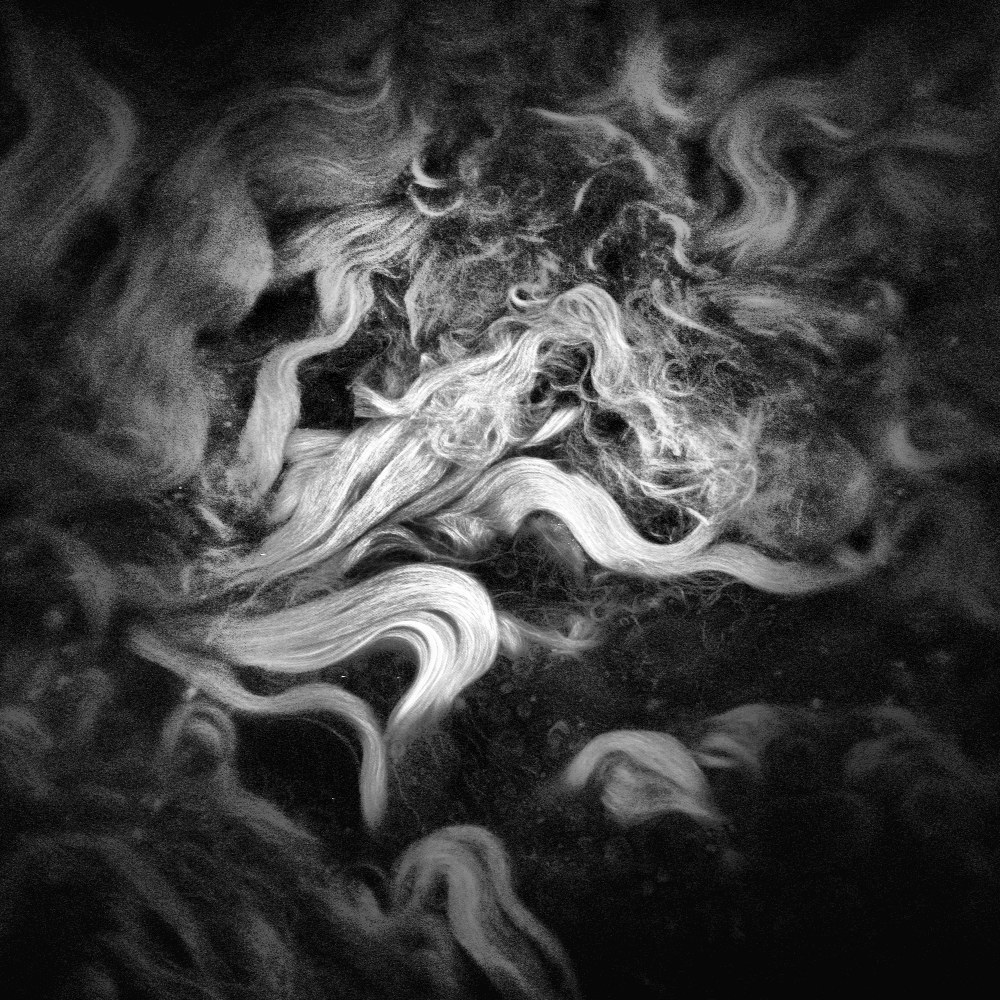
\includegraphics[width=-12.8cm,height=12.8cm]{input.png}};
    \path (0,0,0);
    % input
    \pic[shift={(0,0,0)}] at (0,0,0) {
        Box={
                name=input,
                caption=input,
                xlabel= 1,
                ylabel=258,
                zlabel=\qquad 258,
                fill=,
                height=64,
                width=0.1,
                depth=64
            }
    };
    % conv1
    \pic[shift={(1,0,0)}] at (0,0,0) {
        Box={
                name= conv1,
                caption=conv 3x3,
                xlabel={{"64",""}},
                ylabel=,%258,
                zlabel=258,
                fill=\ConvBNReluColor,
                height=64,
                width=16,
                depth=64
            }
    };
    \draw[connection](-2,0,0) -- node{\midarrow}(conv1-west);
    % MaxPool2d
    \pic[shift={(0,0,0)}] at (conv1-east) {
        Box={
                name=mp1,
                caption=,%Maxpool,
                xlabel={{"64",""}},
                ylabel=,%128,
                zlabel=128,
                fill=\PoolColor,
                height=32,
                width=16,
                depth=32
            }
    };
    \pic[shift={(0,0,0)}] at (mp1-east) {
        Box={
                name=mp2,
                caption=\\[1cm] maxpool,
                xlabel={{"64",""}},
                ylabel=,%64,
                zlabel=64,
                fill=\PoolColor,
                height=16,
                width=16,
                depth=16
            }
    };
    \pic[shift={(0,0,0)}] at (mp2-east) {
        Box={
                name=mp3,
                caption=,%,
                xlabel={{"64",""}},
                ylabel=,%32,
                zlabel=32,
                fill=\PoolColor,
                height=8,
                width=16,
                depth=8
            }
    };

    % CONV 2
    \pic[shift={(2,0,0)}] at (mp3-east) {
        Box={
                name= conv2,
                caption=conv 5x5,
                xlabel={{"64",""}},
                ylabel=,%32,
                zlabel=32,
                fill=\ConvBNReluColor,
                height=8,
                width=16,
                depth=8
            }
    };
    \draw[connection](mp3-east) -- node{\midarrow}(conv2-west);
    % MaxPool2d
    \pic[shift={(0,0,0)}] at (conv2-east) {
        Box={
                name=mp4,
                caption=,%Pooling,
                xlabel={{"64",""}},
                ylabel=,%14,
                zlabel=14,
                fill=\PoolColor,
                height=4,
                width=16,
                depth=4
            }
    };


    % CONV 3
    \pic[shift={(2,0,0)}] at (mp4-east) {
        Box={
                name= conv3,
                caption=conv 3x3,
                xlabel={{"64",""}},
                ylabel=,%14,
                zlabel=14,
                fill=\ConvBNReluColor,
                height=4,
                width=16,
                depth=4
            }
    };
    \draw[connection](mp4-east) -- node{\midarrow}(conv3-west);

    % MaxPool2d
    \pic[shift={(0,0,0)}] at (conv3-east) {
        Box={
                name=mp5,
                caption=,%Pooling,
                xlabel={{"64",""}},
                ylabel=,%7,
                zlabel=7,
                fill=\PoolColor,
                height=2,
                width=16,
                depth=2
            }
    };


    % CONV 4
    \pic[shift={(2,0,0)}] at (mp5-east) {
        Box={
                name= conv4,
                caption=conv 6x6,
                xlabel={{"64",""}},
                ylabel=,%7,
                zlabel=7,
                fill=\ConvBNReluColor,
                height=2,
                width=16,
                depth=2
            }
    };
    \draw[connection](mp5-east) -- node{\midarrow}(conv4-west);

    % \pic[shift={(1,0,0)}] at (conv4-east) {
    %     Box={
    %             name=fc1,
    %             caption=,%,
    %             xlabel={{1, }},
    %             zlabel= 64,
    %             fill=\FcColor,
    %             height=2,
    %             width=2,
    %             depth=16
    %         }
    % };

    % \draw[connection](conv4-east) -- node{\midarrow}(fc1-west);

    \pic[shift={(2,0,0)}] at (conv4-east) {
        Box={
                name=fc2,
                caption=,%,
                xlabel={{1, }},
                zlabel= 64,%$N_\mathrm{nodes}$,
                fill=\FcBNReLUColor,
                height=2,
                width=2,
                depth=64
            }
    };

    \draw[connection](conv4-east) -- node{\midarrow}(fc2-west);

    \pic[shift={(2,0,0)}] at (fc2-east) {
        Box={
                name=fc3,
                caption=,%,
                xlabel={{1, }},
                zlabel=3,
                fill=\FcColor,
                height=2,
                width=2,
                depth=3
            }
    };

    \draw[connection](fc2-east) -- node{\midarrow}(fc3-west);


    \path (fc3-east) ++ (1,0,0) coordinate (output);
    \draw [connection] (fc3-east) -- node {\midarrow} (output);

    % LEGEND
    \matrix [draw,below left] at (current bounding box.south east) {
        \node [convbnrelu,label=right:CONV + BN + ReLU] {}; \\
        \node [mp,label=right:MP 2x2] {};                   \\
        \node [fcbnrelu,label=right:FC + BN + ReLU] {};     \\
        \node [fc,label=right:FC] {};                       \\
    };
\end{tikzpicture}
\end{document}